% latex template
\documentclass[12pt]{article}
\usepackage[utf8]{inputenc}
\usepackage[english]{babel}
\usepackage[margin=1in]{geometry}
\usepackage{caption} % figure captioning
\usepackage{amsmath} % equation tools
\usepackage{amssymb} % math symbols
\usepackage{mathtools} % math rendering improvements
%\usepackage{siunitx} % standard units
\usepackage{graphicx} % add images
%\usepackage{wrapfig} % position images
\usepackage{float} % position images pt.2
%\usepackage[makeroom]{cancel} % cross out text
%\usepackage[version=4]{mhchem} % chemical equations
%\usepackage{multicol} % multiple columns
%\usepackage{pgfplots} % built in plotter
%\pgfplotsset{width=10cm,compat=1.9} % plotter settings
\usepackage{hyperref} % table of contents links
\usepackage{indentfirst} % indent first paragraph after section

\hypersetup{
    colorlinks,
    citecolor=black,
    filecolor=black,
    linkcolor=black,
    urlcolor=black
}

\renewcommand{\baselinestretch}{1.5} % line spacing
\newcommand{\fline}{\par\noindent\rule{\textwidth}{0.1pt}} % horizontal line (wide)

\title{EE TITLE}
\author{Bryan Deng}
\date{}

\begin{document}

\maketitle
\newpage
\tableofcontents
\newpage

\section{Background Information}

\subsection{Machine Learning and its Applications}

Machine learning (ML) is a branch of artificial intelligence that uses large datasets and algorithms to mimic the way humans learn and improve accuracy over time \cite{what_is_ml_ibm}. Since its debut in 1952, it has been steadily gaining popularity for its abilities in recognizing patterns and continuous learning. Machine learning powers many of the applications we use on a daily basis, including chatbots, language translation tools, and social media feeds \cite{what_is_ml_mit}.

Where machine learning shines is in its ability to solve problems that would typically be either impossible for impractical for traditional algorithms. Furthermore, machine learning models are able to generalize these solutions and apply them to additional problems it has never encountered before.

In short, machine learning is a combination of computer science, statistics, and optimization. It uses knowledge from different fields to ``teach'' computers to complete tasks. As the model looks at more and more data, it starts to recognize patterns among it and optimizes itself.

\subsection{Decision Trees}

When most think about machine learning, the first thing that comes to mind are neural networks. Neural networks, which are abstractly complex yet powerful algorithms, only make up one subfield of machine learning itself, called \textit{deep learning}. However, there exist several other branches of machine learning, such as \textit{supervised learning}, the main focus of this paper. The most well known model within supervised learning has to be the decision tree. They are binary trees which employ a straightforward \textit{if-else} flow to classify data.

\begin{figure}[H]
    \centering
    \fbox{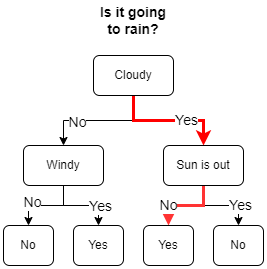
\includegraphics[scale=0.7]{figs/decision_tree.png}}
    \caption{Decision Tree Diagram}
    \label{fig:decisiontree}
\end{figure}

\hyperref[fig:decisiontree]{Figure 1} shows a simple decision tree to predict whether it will rain based on other weather conditions. Given a cloudy day with no sun, the model will predict that it will rain, as outlined by the red lines on the diagram. The anatomy of a decision tree consists of several parts \cite{dt_skl_doc}:

\begin{itemize}
    \item \textbf{Node}: cells that contain data. A tree is made of several nodes connected by edges.
    \begin{itemize}
        \item \textbf{Root node}: the single node at the very top of the tree.
        \item \textbf{Split node}: a split node splits into two other child nodes based on a feature and split value.
        \item \textbf{Leaf node}: a node at the end of a tree; it does not split into further nodes.
        \item \textbf{Child node}: the nodes that follow split nodes.
    \end{itemize}
    \item \textbf{Feature}: an individual characteristic of a dataset \cite{pattern_recognition_ml}, the $i$th feature is represented as $x_i$.
    \item \textbf{Split Value}: a value that classifies any data that the node encounters (e.g. $x_i \le2.7$)
\end{itemize}

The main computational problem with decision trees is how first construct, then optimize them. If we were to generate a random decision tree structure, it could potentially become very large and unnecessarily complex, taking up extra resources in computation. And if we were to simply assign each node a random feature and split value, it is very unlikely the model will perform well in predictions.

The approach used in vanilla decision trees is a greedy top-down algorithm that builds nodes, assigning it features and split values as it moves down the tree \cite{dt_induction}. Other well-established algorithms for constructing decision trees include random forests and gradient boosting. This paper aims to investigate a new decision tree construction and optimization algorithm by employing the genetic algorithm.

\subsection{Genetic Algorithm}

Taking a page straight out of Darwin's theory of evolution, genetic algorithms employ the principle of \textit{survival of the fittest}. It generates populations of algorithms or models that evolve and reproduce over time based on a set of criteria, improving on performance. Each \textit{individual} of the population is represented by a form of data structure. Each piece of data can be paralleled to a gene, which when all combined describes the behavior of the individual \cite{intro_to_ga}. The steps of the genetic algorithm are as follows:

\begin{itemize}
    \item \textbf{Initialization}: an initial population is generated with random genes using a set of preset hyperparameters.
    \item \textbf{Fitness evaluation}: a score given to each individual in the population based on how well it performs for the problem.
    \item \textbf{Selection}: a process to select the individuals that will carry forward or reproduce for the next generation, usually based on fitness.
    \item \textbf{Crossover}: a process to either sexually or asexually reproduce individuals for the next generation based on the previous generation.
    \item \textbf{Mutation}: randomly altering genes of an individual to maintain diversity and encourage further exploration of the solution space.
    \item \textbf{Termination}: a set of criterion to determine when reproduction for new generations should stop.
\end{itemize}

The species in real life which benefit the most from evolution are those that are able to maintain diversity. With diversity, they can overcome external problems like diseases or natural disasters. Similarly, the genetic algorithm puts a strong emphasis on diversity, so it can explore a large solution space and escape falling into a local minimum. Diversity is achieved with several stages of randomness introduced in each generation, in selection, crossover and mutation.

\subsection{Evolutionary Decision Tree}

An evolutionary decision tree (EDT) uses a genetic algorithm to optimize a decision tree.

\section{Experimental Methodology}

\section{Data Analysis}

\section{Error Analysis}

\section{Conclusion}

\section{Appendix}

\bibliographystyle{plain}
\bibliography{refs}

\end{document}

